\chapter{Protein Location Relation Extraction: Materials \& Methods}\label{chapter:methods}
\newcommand*{\xml}[1]{\texttt{<#1>}}
\section{Task Definition}

This chapter explains the method developed to extract Protein-Location relations from Biomedical Text. This task of relation extraction comes under the broad category of Natural Language Processing as explained in the section \ref{sec:RE}. The task of extraction of Protein-Location relations can be formally described as follows:

Given a piece of text that contains two entity mentions i.e. Protein and Location, the task of relation extraction method is to decide if the text contains enough evidence for semantic relationship between these two entities. Formally, let $r=(t,arg_1,arg_2)$ denote a relationship instance where $t$ is a piece of text, $arg_1$ \& $arg_2$  are entity mentions contained in text $t$ and $arg_1$ precedes $arg_2$ in the text. Given a set of relations $\left\lbrace r_i \right\rbrace$ such that every relation instance has label $l \in \left\lbrace-1,1\right\rbrace$, our task is to learn a function that can predict the label $l$ for new relation instances whose label are not known. Note that $t$ can simply be a piece of text or it may also contain structured information such as parse tree and dependency graphs. For entity mentions $arg_1$ and $arg_2$, either of them can represent a protein or a location entity.
 
% Following section to be deleted, to be shifted to introduction
\section{State of the art in BioNLP'09}

% where should I put that
We tried to replicate the result of Björne et.al. to get started with our model.The selection of features in our model is heavily influenced by features from the model of Björne et.al.

\section{Method for Protein-Location Relation Extraction}

I will describe the method that I developed for extraction of protein-location relations in subsequent sections. Here is the overview of sections in this chapter: Section \ref{sec:ssModeldsModel} explains the motivation behind creating more than 1 machine learning model. Section \ref{sec:pipeline} outlines the flow of information in this process. Section \ref{sec:models} introduces the machine learning models developed for the task of relationship extraction. Section \ref{sec:graphRep} explains the actual representation of data in the model. The process of feature extraction and feature selection is explained in section \ref{sec:featExp} and \ref{sec:featSel} respectively.

The training methodologies and procedures are explained in section \ref{sec:training}. Section \ref{sec:experiments} talks about all different experiments tried and their effect on the overall method and section \ref{sec:tools} concludes the explanation about the method.

\section{Same sentence model \& different sentence model}\label{sec:ssModeldsModel}

The protein-location relation is a relation between a protein entity and a location entity present in the text. Both protein and location entity may reside in the single sentence or it might happen that these entities are in different sentences. In the case of LocText corpus, as pointed out in section \ref{sec:corpusStats}, around 60\% of the protein-location relations are same sentence relations i.e., both protein entity and location entity are present in a single sentence. However, a large portion of protein location relations (nearly 40\%) are different sentence relations in which the participating entities are not present in a single sentence. This is the motivation that we decided to build a relation extraction method which can extract relations from single sentence as well as from different sentences. The semantic relationship between protein and location in the case of different sentence relations with large sentence distance might be difficult to extract and hence, I tried to focus only on those different sentence relations which have a sentence distance of 1 i.e., the protein and location entities are not present in the same sentence but are found in neighboring sentence.

Therefore, we decided to build two models viz. same sentence model (abbreviated as SSModel hereafter) and different sentence model (abbreviated as DSModel hereafter). SSModel tries to extract the relations present in a single sentence whereas DSModel tries to extract different sentence relations.

\section{Method pipeline}\label{sec:pipeline}

%- Explain the whole pipeline 
%- Corpus-->Sentence Segmentation-->Tokenization-->Syntactic & dependency Parsing-->Graph Representation-->  Feature Extraction --> ML Model training -->Classification on Test
%- Put a nice picture explaining the pipeline



The overall relation extraction method consists of following major stages:

\begin{enumerate}

\item \textbf{Data collection \& Corpus creation}

For LocText corpus, the annotated data is present in JSON files that can be downloaded through the web-interface. However, the JSON files contain only annotations and not the actual text. The actual text is present in separate set of HTML files. Every JSON or HTML file corresponds to particular PubMedID. In every HTML file, the data is divided into title and abstract. To avoid reading from plain files repeatedly, I decided to create a XML file containing all corpus data along with annotations and structural details like parse tree, dependency graphs etc.

\begin{figure}
\centering
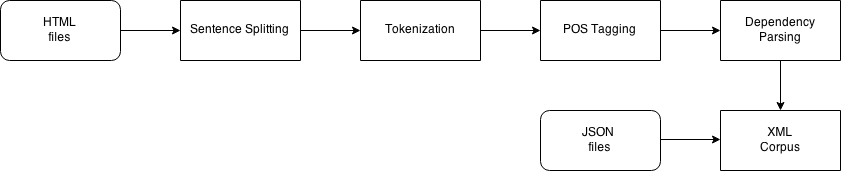
\includegraphics[scale=0.4]{figures/Corpus_Creation.png}
\caption{The process of creating a XML corpus file}\label{fig:corpusCreation}
\end{figure}

Figure \ref{fig:corpusCreation} outlines the process  of corpus creation. The data read from HTML files is parsed using Stanford CoreNLP pipeline [CITE:STANFORD CORENLP]. The text from HTML files which consist of title and abstract is initially segmented into sentences. Every sentences is then split into tokens (tokenization). The part of speech tag for every token is also computed. Finally, the dependency relations between tokens are computed.

All the unstructured (plain text) and structured (sentences, tokens, POS tags, dependencies) information is then combined with annotations present in JSON files and written to the XML corpus file.

\begin{figure}
\centering
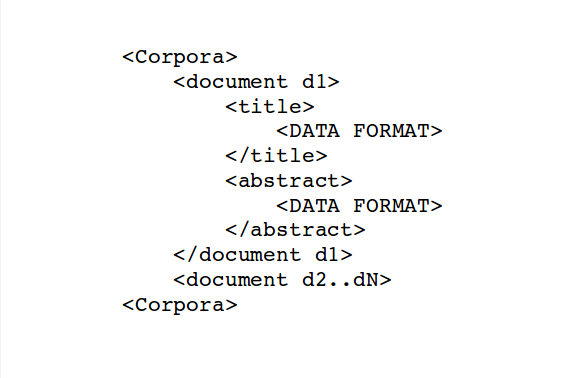
\includegraphics[scale=0.4]{figures/XMLSchema1.png}
\caption{Coarse XML schema}\label{fig:XMLSchema1}
\end{figure}

The coarse XML schema of the corpus XML file can be shown in the fig. \ref{fig:XMLSchema1}.The "DATA FORMAT" which is common to both title and abstract node can be elaborated as in fig. \ref{fig:XMLSchema2}.

\begin{figure}
\centering
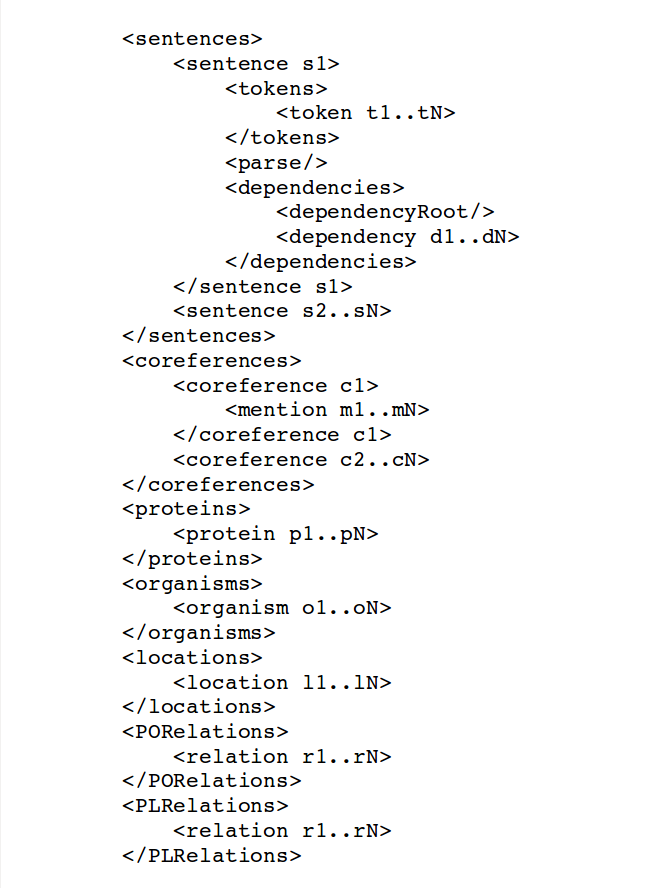
\includegraphics[scale=0.4]{figures/XMLSchema2.png}
\caption{Data format common to title and abstract node}\label{fig:XMLSchema2}
\end{figure}

\item \textbf{Training \& evaluating same sentence model}
\item \textbf{Training \& evaluating different sentence model}
\item \textbf{Combined evaluation}
\end{enumerate}

\section{Machine Learning Models}\label{sec:models}
% Talk about different models here so that there is no confusion ahead

\subsection{SameSentenceModel}

\subsection{DiffSentenceModel}

\section{Graph representation} \label{sec:graphRep}
% Details about graph representation along with nice explanatory picture

\subsection{Graph representation for SameSentenceModel}

\subsection{Graph representation for DiffSentenceModel}

\section{Feature extraction}\label{sec:featExp}

\subsection{Feature extraction for SameSentenceModel}

\subsection{Feature extraction for DiffSentenceModel}

\section{Feature Selection}\label{sec:featSel}

%Write some of the results found out from in Joachim's paper [Text categorization with SVM]
%
%**This is a very important property that has got to be known that in text categorization using SVM, there are only few irrelevant features.
%
%When ranked according to Binary information gain, see Figure 1, removal of high ranking features doesnot take away a lot of information. This also means that even features ranked lowest still contain considerable information and are somewhat relevant.
%
%TODO: See how to calculate binary information gain for a feature/set of features.***

\section{Training, Cross validation and Classification}\label{sec:training}

\section{Experiments that worked and that did not work}\label{sec:experiments}

\subsection{Experimentation for SameSentModel}

- Removing sentences which had no proteins improved the performance
- Using different kernels did not work

\subsection{Experimentation for DiffSentModel}

- Using extra information from the document such as shortform longform pairs decreased the performance since it added more FP's (15) than TP's (1). It seems that this rule was nicely followed during annotation

\subsection{Experimentation with different kernels}

\section{Tools used}\label{sec:tools}
